\documentclass[1p]{elsarticle_modified}
%\bibliographystyle{elsarticle-num}

%\usepackage[colorlinks]{hyperref}
%\usepackage{abbrmath_seonhwa} %\Abb, \Ascr, \Acal ,\Abf, \Afrak
\usepackage{amsfonts}
\usepackage{amssymb}
\usepackage{amsmath}
\usepackage{amsthm}
\usepackage{scalefnt}
\usepackage{amsbsy}
\usepackage{kotex}
\usepackage{caption}
\usepackage{subfig}
\usepackage{color}
\usepackage{graphicx}
\usepackage{xcolor} %% white, black, red, green, blue, cyan, magenta, yellow
\usepackage{float}
\usepackage{setspace}
\usepackage{hyperref}

\usepackage{tikz}
\usetikzlibrary{arrows}

\usepackage{multirow}
\usepackage{array} % fixed length table
\usepackage{hhline}

%%%%%%%%%%%%%%%%%%%%%
\makeatletter
\renewcommand*\env@matrix[1][\arraystretch]{%
	\edef\arraystretch{#1}%
	\hskip -\arraycolsep
	\let\@ifnextchar\new@ifnextchar
	\array{*\c@MaxMatrixCols c}}
\makeatother %https://tex.stackexchange.com/questions/14071/how-can-i-increase-the-line-spacing-in-a-matrix
%%%%%%%%%%%%%%%

\usepackage[normalem]{ulem}

\newcommand{\msout}[1]{\ifmmode\text{\sout{\ensuremath{#1}}}\else\sout{#1}\fi}
%SOURCE: \msout is \stkout macro in https://tex.stackexchange.com/questions/20609/strikeout-in-math-mode

\newcommand{\cancel}[1]{
	\ifmmode
	{\color{red}\msout{#1}}
	\else
	{\color{red}\sout{#1}}
	\fi
}

\newcommand{\add}[1]{
	{\color{blue}\uwave{#1}}
}

\newcommand{\replace}[2]{
	\ifmmode
	{\color{red}\msout{#1}}{\color{blue}\uwave{#2}}
	\else
	{\color{red}\sout{#1}}{\color{blue}\uwave{#2}}
	\fi
}

\newcommand{\Sol}{\mathcal{S}} %segment
\newcommand{\D}{D} %diagram
\newcommand{\A}{\mathcal{A}} %arc


%%%%%%%%%%%%%%%%%%%%%%%%%%%%%5 test

\def\sl{\operatorname{\textup{SL}}(2,\Cbb)}
\def\psl{\operatorname{\textup{PSL}}(2,\Cbb)}
\def\quan{\mkern 1mu \triangleright \mkern 1mu}

\theoremstyle{definition}
\newtheorem{thm}{Theorem}[section]
\newtheorem{prop}[thm]{Proposition}
\newtheorem{lem}[thm]{Lemma}
\newtheorem{ques}[thm]{Question}
\newtheorem{cor}[thm]{Corollary}
\newtheorem{defn}[thm]{Definition}
\newtheorem{exam}[thm]{Example}
\newtheorem{rmk}[thm]{Remark}
\newtheorem{alg}[thm]{Algorithm}

\newcommand{\I}{\sqrt{-1}}
\begin{document}

%\begin{frontmatter}
%
%\title{Boundary parabolic representations of knots up to 8 crossings}
%
%%% Group authors per affiliation:
%\author{Yunhi Cho} 
%\address{Department of Mathematics, University of Seoul, Seoul, Korea}
%\ead{yhcho@uos.ac.kr}
%
%
%\author{Seonhwa Kim} %\fnref{s_kim}}
%\address{Center for Geometry and Physics, Institute for Basic Science, Pohang, 37673, Korea}
%\ead{ryeona17@ibs.re.kr}
%
%\author{Hyuk Kim}
%\address{Department of Mathematical Sciences, Seoul National University, Seoul 08826, Korea}
%\ead{hyukkim@snu.ac.kr}
%
%\author{Seokbeom Yoon}
%\address{Department of Mathematical Sciences, Seoul National University, Seoul, 08826,  Korea}
%\ead{sbyoon15@snu.ac.kr}
%
%\begin{abstract}
%We find all boundary parabolic representation of knots up to 8 crossings.
%
%\end{abstract}
%\begin{keyword}
%    \MSC[2010] 57M25 
%\end{keyword}
%
%\end{frontmatter}

%\linenumbers
%\tableofcontents
%
\newcommand\colored[1]{\textcolor{white}{\rule[-0.35ex]{0.8em}{1.4ex}}\kern-0.8em\color{red} #1}%
%\newcommand\colored[1]{\textcolor{white}{ #1}\kern-2.17ex	\textcolor{white}{ #1}\kern-1.81ex	\textcolor{white}{ #1}\kern-2.15ex\color{red}#1	}

{\Large $\underline{12n_{0109}~(K12n_{0109})}$}

\setlength{\tabcolsep}{10pt}
\renewcommand{\arraystretch}{1.6}
\vspace{1cm}\begin{tabular}{m{100pt}>{\centering\arraybackslash}m{274pt}}
\multirow{5}{120pt}{
	\centering
	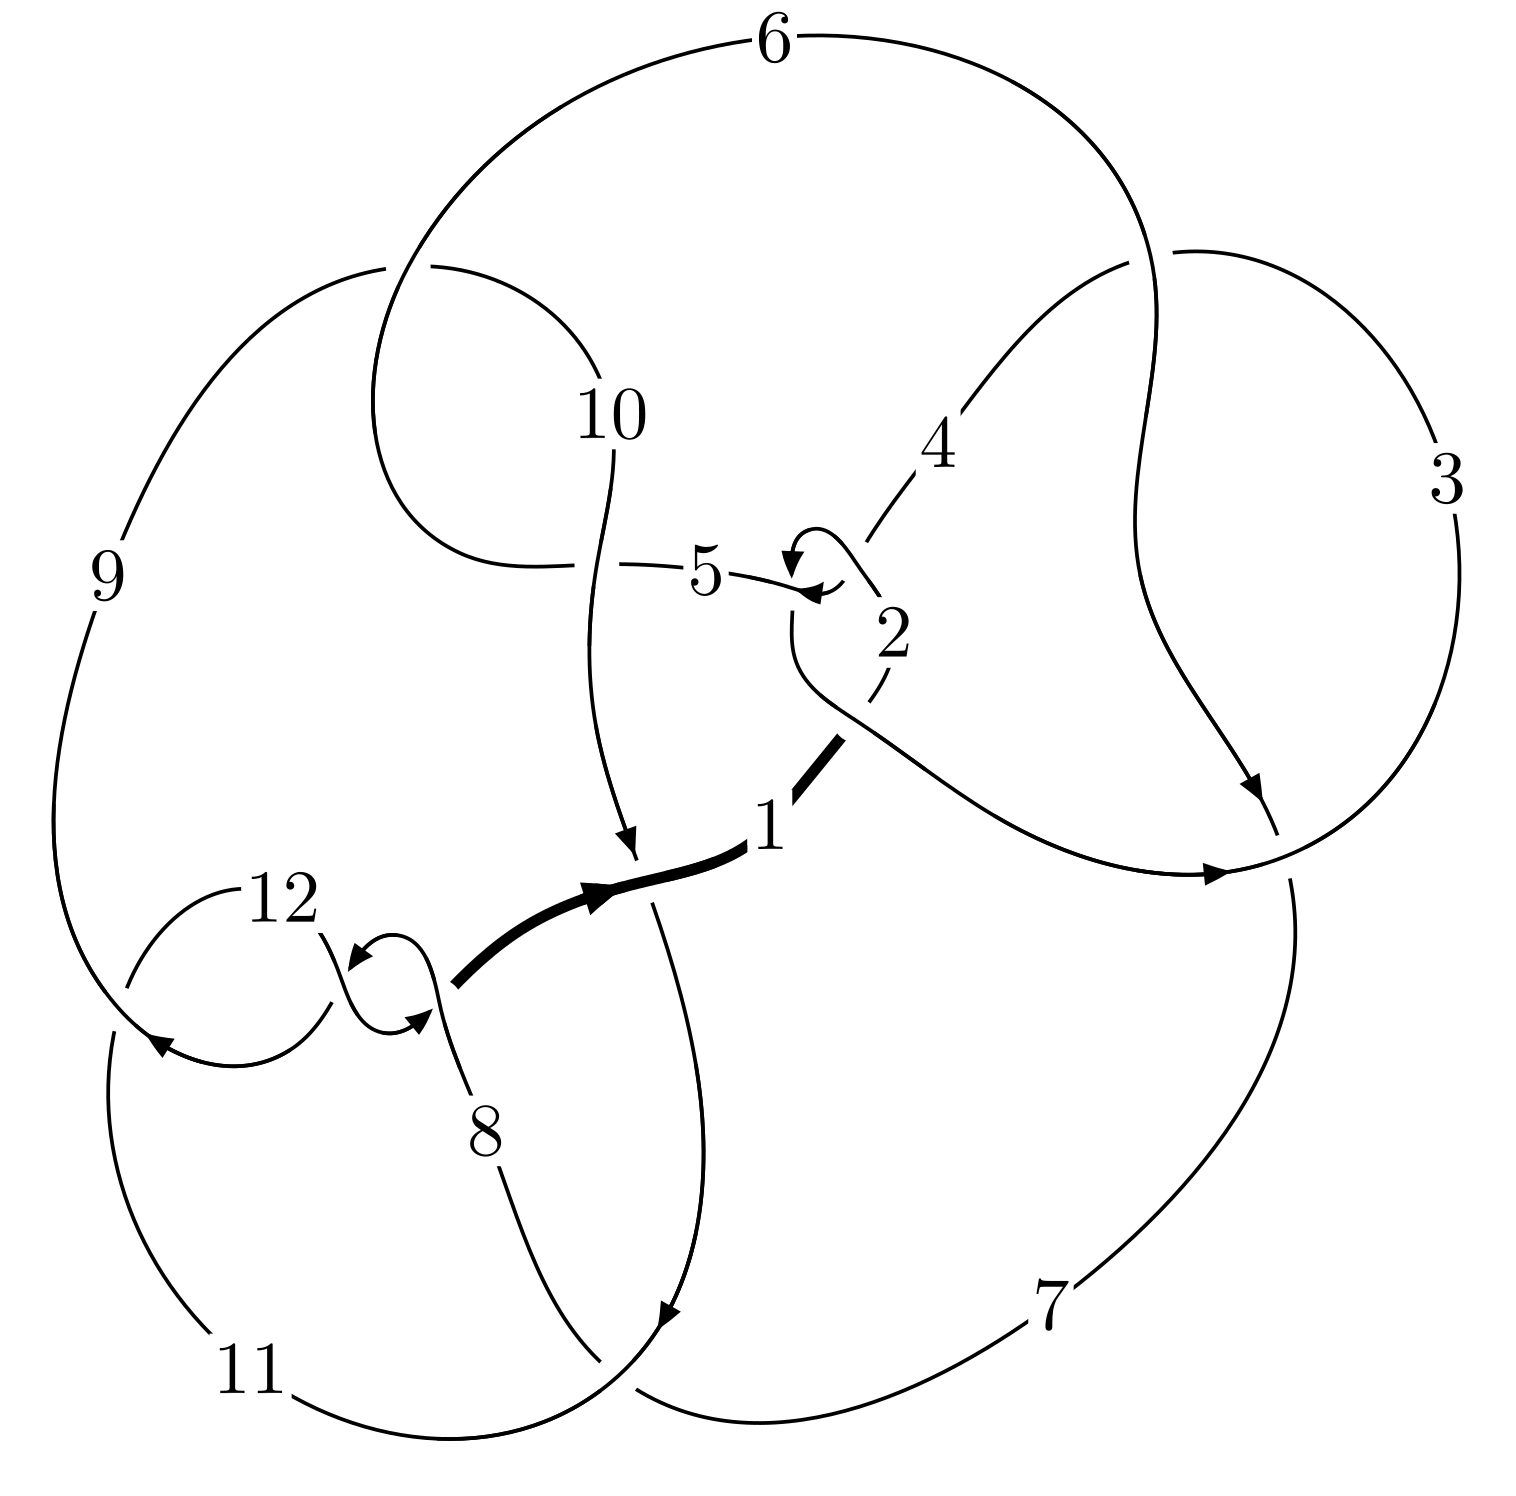
\includegraphics[width=112pt]{../../../GIT/diagram.site/Diagrams/png/2198_12n_0109.png}\\
\ \ \ A knot diagram\footnotemark}&
\allowdisplaybreaks
\textbf{Linearized knot diagam} \\
\cline{2-2}
 &
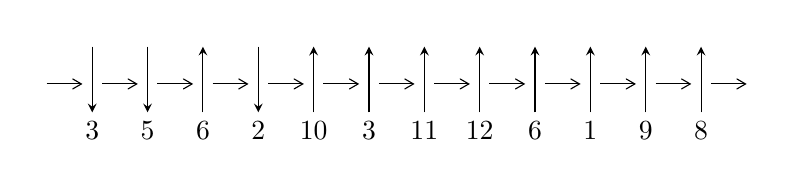
\begin{tikzpicture}[x=20pt, y=17pt]
	% nodes
	\node (C0) at (0, 0) {};
	\node (C1) at (1, 0) {};
	\node (C1U) at (1, +1) {};
	\node (C1D) at (1, -1) {3};

	\node (C2) at (2, 0) {};
	\node (C2U) at (2, +1) {};
	\node (C2D) at (2, -1) {5};

	\node (C3) at (3, 0) {};
	\node (C3U) at (3, +1) {};
	\node (C3D) at (3, -1) {6};

	\node (C4) at (4, 0) {};
	\node (C4U) at (4, +1) {};
	\node (C4D) at (4, -1) {2};

	\node (C5) at (5, 0) {};
	\node (C5U) at (5, +1) {};
	\node (C5D) at (5, -1) {10};

	\node (C6) at (6, 0) {};
	\node (C6U) at (6, +1) {};
	\node (C6D) at (6, -1) {3};

	\node (C7) at (7, 0) {};
	\node (C7U) at (7, +1) {};
	\node (C7D) at (7, -1) {11};

	\node (C8) at (8, 0) {};
	\node (C8U) at (8, +1) {};
	\node (C8D) at (8, -1) {12};

	\node (C9) at (9, 0) {};
	\node (C9U) at (9, +1) {};
	\node (C9D) at (9, -1) {6};

	\node (C10) at (10, 0) {};
	\node (C10U) at (10, +1) {};
	\node (C10D) at (10, -1) {1};

	\node (C11) at (11, 0) {};
	\node (C11U) at (11, +1) {};
	\node (C11D) at (11, -1) {9};

	\node (C12) at (12, 0) {};
	\node (C12U) at (12, +1) {};
	\node (C12D) at (12, -1) {8};
	\node (C13) at (13, 0) {};

	% arrows
	\draw[->,>={angle 60}]
	(C0) edge (C1) (C1) edge (C2) (C2) edge (C3) (C3) edge (C4) (C4) edge (C5) (C5) edge (C6) (C6) edge (C7) (C7) edge (C8) (C8) edge (C9) (C9) edge (C10) (C10) edge (C11) (C11) edge (C12) (C12) edge (C13) ;	\draw[->,>=stealth]
	(C1U) edge (C1D) (C2U) edge (C2D) (C3D) edge (C3U) (C4U) edge (C4D) (C5D) edge (C5U) (C6D) edge (C6U) (C7D) edge (C7U) (C8D) edge (C8U) (C9D) edge (C9U) (C10D) edge (C10U) (C11D) edge (C11U) (C12D) edge (C12U) ;
	\end{tikzpicture} \\
\hhline{~~} \\& 
\textbf{Solving Sequence} \\ \cline{2-2} 
 &
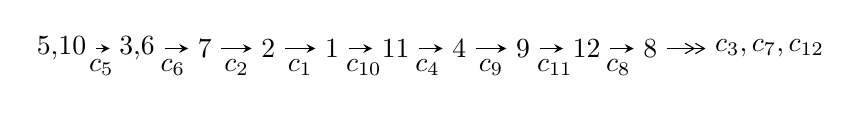
\begin{tikzpicture}[x=23pt, y=7pt]
	% node
	\node (A0) at (-1/8, 0) {5,10};
	\node (A1) at (17/16, 0) {3,6};
	\node (A2) at (17/8, 0) {7};
	\node (A3) at (25/8, 0) {2};
	\node (A4) at (33/8, 0) {1};
	\node (A5) at (41/8, 0) {11};
	\node (A6) at (49/8, 0) {4};
	\node (A7) at (57/8, 0) {9};
	\node (A8) at (65/8, 0) {12};
	\node (A9) at (73/8, 0) {8};
	\node (C1) at (1/2, -1) {$c_{5}$};
	\node (C2) at (13/8, -1) {$c_{6}$};
	\node (C3) at (21/8, -1) {$c_{2}$};
	\node (C4) at (29/8, -1) {$c_{1}$};
	\node (C5) at (37/8, -1) {$c_{10}$};
	\node (C6) at (45/8, -1) {$c_{4}$};
	\node (C7) at (53/8, -1) {$c_{9}$};
	\node (C8) at (61/8, -1) {$c_{11}$};
	\node (C9) at (69/8, -1) {$c_{8}$};
	\node (A10) at (11, 0) {$c_{3},c_{7},c_{12}$};

	% edge
	\draw[->,>=stealth]	
	(A0) edge (A1) (A1) edge (A2) (A2) edge (A3) (A3) edge (A4) (A4) edge (A5) (A5) edge (A6) (A6) edge (A7) (A7) edge (A8) (A8) edge (A9) ;
	\draw[->>,>={angle 60}]	
	(A9) edge (A10);
\end{tikzpicture} \\ 

\end{tabular} \\

\footnotetext{
The image of knot diagram is generated by the software ``\textbf{Draw programme}" developed by Andrew Bartholomew(\url{http://www.layer8.co.uk/maths/draw/index.htm\#Running-draw}), where we modified some parts for our purpose(\url{https://github.com/CATsTAILs/LinksPainter}).
}\phantom \\ \newline 
\centering \textbf{Ideals for irreducible components\footnotemark of $X_{\text{par}}$} 
 
\begin{align*}
I^u_{1}&=\langle 
6.35220\times10^{79} u^{55}+2.03304\times10^{79} u^{54}+\cdots+6.01137\times10^{80} b+5.14680\times10^{80},\\
\phantom{I^u_{1}}&\phantom{= \langle  }-6.55161\times10^{79} u^{55}-5.38999\times10^{80} u^{54}+\cdots+6.01137\times10^{80} a-2.37369\times10^{81},\;u^{56}+2 u^{55}+\cdots- u-1\rangle \\
I^u_{2}&=\langle 
b+1,\;-2 u^2+a+u-4,\;u^3+2 u+1\rangle \\
I^u_{3}&=\langle 
b+1,\;2 u^3- u^2+a+3 u-2,\;u^4- u^3+2 u^2-2 u+1\rangle \\
\\
\end{align*}
\raggedright * 3 irreducible components of $\dim_{\mathbb{C}}=0$, with total 63 representations.\\
\footnotetext{All coefficients of polynomials are rational numbers. But the coefficients are sometimes approximated in decimal forms when there is not enough margin.}
\newpage
\renewcommand{\arraystretch}{1}
\centering \section*{I. $I^u_{1}= \langle 6.35\times10^{79} u^{55}+2.03\times10^{79} u^{54}+\cdots+6.01\times10^{80} b+5.15\times10^{80},\;-6.55\times10^{79} u^{55}-5.39\times10^{80} u^{54}+\cdots+6.01\times10^{80} a-2.37\times10^{81},\;u^{56}+2 u^{55}+\cdots- u-1 \rangle$}
\flushleft \textbf{(i) Arc colorings}\\
\begin{tabular}{m{7pt} m{180pt} m{7pt} m{180pt} }
\flushright $a_{5}=$&$\begin{pmatrix}1\\0\end{pmatrix}$ \\
\flushright $a_{10}=$&$\begin{pmatrix}0\\u\end{pmatrix}$ \\
\flushright $a_{3}=$&$\begin{pmatrix}0.108987 u^{55}+0.896633 u^{54}+\cdots+0.394522 u+3.94866\\-0.105670 u^{55}-0.0338199 u^{54}+\cdots-0.859496 u-0.856178\end{pmatrix}$ \\
\flushright $a_{6}=$&$\begin{pmatrix}1\\- u^2\end{pmatrix}$ \\
\flushright $a_{7}=$&$\begin{pmatrix}-0.146691 u^{55}+0.118799 u^{54}+\cdots-1.49357 u-0.175836\\-0.0587371 u^{55}-0.170653 u^{54}+\cdots-0.0940050 u-0.334345\end{pmatrix}$ \\
\flushright $a_{2}=$&$\begin{pmatrix}0.00331723 u^{55}+0.862813 u^{54}+\cdots-0.464973 u+3.09249\\-0.105670 u^{55}-0.0338199 u^{54}+\cdots-0.859496 u-0.856178\end{pmatrix}$ \\
\flushright $a_{1}=$&$\begin{pmatrix}-0.228248 u^{55}-0.101789 u^{54}+\cdots-1.32208 u-0.0980010\\0.0815574 u^{55}+0.220588 u^{54}+\cdots-0.171485 u-0.0778350\end{pmatrix}$ \\
\flushright $a_{11}=$&$\begin{pmatrix}-0.00788014 u^{55}+0.337184 u^{54}+\cdots+0.0774386 u+0.935949\\0.0508844 u^{55}+0.122185 u^{54}+\cdots+0.834455 u-0.157223\end{pmatrix}$ \\
\flushright $a_{4}=$&$\begin{pmatrix}0.0740743 u^{55}+0.802152 u^{54}+\cdots+0.322672 u+3.77114\\-0.134670 u^{55}-0.112515 u^{54}+\cdots-0.799927 u-0.831523\end{pmatrix}$ \\
\flushright $a_{9}=$&$\begin{pmatrix}- u\\u^3+u\end{pmatrix}$ \\
\flushright $a_{12}=$&$\begin{pmatrix}-0.152843 u^{55}+0.00107466 u^{54}+\cdots+0.363574 u+1.27464\\0.288502 u^{55}+0.643234 u^{54}+\cdots+0.739466 u-0.449730\end{pmatrix}$ \\
\flushright $a_{8}=$&$\begin{pmatrix}0.103064 u^{55}+0.314464 u^{54}+\cdots-0.906044 u-1.96765\\-0.000335653 u^{55}-0.103672 u^{54}+\cdots-0.200689 u-0.573235\end{pmatrix}$\\&\end{tabular}
\flushleft \textbf{(ii) Obstruction class $= -1$}\\~\\
\flushleft \textbf{(iii) Cusp Shapes $= -2.60373 u^{55}+0.0539183 u^{54}+\cdots+14.8197 u+24.5026$}\\~\\
\newpage\renewcommand{\arraystretch}{1}
\flushleft \textbf{(iv) u-Polynomials at the component}\newline \\
\begin{tabular}{m{50pt}|m{274pt}}
Crossings & \hspace{64pt}u-Polynomials at each crossing \\
\hline $$\begin{aligned}c_{1}\end{aligned}$$&$\begin{aligned}
&u^{56}+20 u^{55}+\cdots+436 u+1
\end{aligned}$\\
\hline $$\begin{aligned}c_{2},c_{4}\end{aligned}$$&$\begin{aligned}
&u^{56}-8 u^{55}+\cdots+20 u-1
\end{aligned}$\\
\hline $$\begin{aligned}c_{3},c_{6}\end{aligned}$$&$\begin{aligned}
&u^{56}+7 u^{55}+\cdots-192 u+128
\end{aligned}$\\
\hline $$\begin{aligned}c_{5},c_{9}\end{aligned}$$&$\begin{aligned}
&u^{56}-2 u^{55}+\cdots+u-1
\end{aligned}$\\
\hline $$\begin{aligned}c_{7}\end{aligned}$$&$\begin{aligned}
&u^{56}-2 u^{55}+\cdots+24 u+36
\end{aligned}$\\
\hline $$\begin{aligned}c_{8},c_{11},c_{12}\end{aligned}$$&$\begin{aligned}
&u^{56}+2 u^{55}+\cdots+3 u+1
\end{aligned}$\\
\hline $$\begin{aligned}c_{10}\end{aligned}$$&$\begin{aligned}
&u^{56}+14 u^{55}+\cdots+663 u+99
\end{aligned}$\\
\hline
\end{tabular}\\~\\
\newpage\renewcommand{\arraystretch}{1}
\flushleft \textbf{(v) Riley Polynomials at the component}\newline \\
\begin{tabular}{m{50pt}|m{274pt}}
Crossings & \hspace{64pt}Riley Polynomials at each crossing \\
\hline $$\begin{aligned}c_{1}\end{aligned}$$&$\begin{aligned}
&y^{56}+40 y^{55}+\cdots-177984 y+1
\end{aligned}$\\
\hline $$\begin{aligned}c_{2},c_{4}\end{aligned}$$&$\begin{aligned}
&y^{56}-20 y^{55}+\cdots-436 y+1
\end{aligned}$\\
\hline $$\begin{aligned}c_{3},c_{6}\end{aligned}$$&$\begin{aligned}
&y^{56}-45 y^{55}+\cdots-749568 y+16384
\end{aligned}$\\
\hline $$\begin{aligned}c_{5},c_{9}\end{aligned}$$&$\begin{aligned}
&y^{56}+14 y^{55}+\cdots-5 y+1
\end{aligned}$\\
\hline $$\begin{aligned}c_{7}\end{aligned}$$&$\begin{aligned}
&y^{56}-6 y^{55}+\cdots+8424 y+1296
\end{aligned}$\\
\hline $$\begin{aligned}c_{8},c_{11},c_{12}\end{aligned}$$&$\begin{aligned}
&y^{56}+50 y^{55}+\cdots-5 y+1
\end{aligned}$\\
\hline $$\begin{aligned}c_{10}\end{aligned}$$&$\begin{aligned}
&y^{56}+2 y^{55}+\cdots-93069 y+9801
\end{aligned}$\\
\hline
\end{tabular}\\~\\
\newpage\flushleft \textbf{(vi) Complex Volumes and Cusp Shapes}
$$\begin{array}{c|c|c}  
\text{Solutions to }I^u_{1}& \I (\text{vol} + \sqrt{-1}CS) & \text{Cusp shape}\\
 \hline 
\begin{aligned}
u &= \phantom{-}0.434045 + 0.764937 I \\
a &= \phantom{-}0.226290 - 1.290380 I \\
b &= -0.870790 + 0.961543 I\end{aligned}
 & -5.25808 + 6.99458 I & -0.29764 - 8.96864 I \\ \hline\begin{aligned}
u &= \phantom{-}0.434045 - 0.764937 I \\
a &= \phantom{-}0.226290 + 1.290380 I \\
b &= -0.870790 - 0.961543 I\end{aligned}
 & -5.25808 - 6.99458 I & -0.29764 + 8.96864 I \\ \hline\begin{aligned}
u &= \phantom{-}0.607815 + 0.613715 I \\
a &= \phantom{-}0.265971 - 1.018000 I \\
b &= -0.230951 + 0.717761 I\end{aligned}
 & -2.75732 + 1.48664 I & \phantom{-}3.92275 - 4.13753 I \\ \hline\begin{aligned}
u &= \phantom{-}0.607815 - 0.613715 I \\
a &= \phantom{-}0.265971 + 1.018000 I \\
b &= -0.230951 - 0.717761 I\end{aligned}
 & -2.75732 - 1.48664 I & \phantom{-}3.92275 + 4.13753 I \\ \hline\begin{aligned}
u &= -0.451362 + 0.714754 I \\
a &= \phantom{-}0.234053 + 1.284310 I \\
b &= -0.750580 - 0.842936 I\end{aligned}
 & -0.27969 - 3.79973 I & \phantom{-}5.42430 + 9.11034 I \\ \hline\begin{aligned}
u &= -0.451362 - 0.714754 I \\
a &= \phantom{-}0.234053 - 1.284310 I \\
b &= -0.750580 + 0.842936 I\end{aligned}
 & -0.27969 + 3.79973 I & \phantom{-}5.42430 - 9.11034 I \\ \hline\begin{aligned}
u &= -0.862715 + 0.810503 I \\
a &= -0.398734 + 0.878095 I \\
b &= \phantom{-}0.522743 - 1.197170 I\end{aligned}
 & \phantom{-}1.24825 - 8.12321 I & \phantom{-0.000000 } 0 \\ \hline\begin{aligned}
u &= -0.862715 - 0.810503 I \\
a &= -0.398734 - 0.878095 I \\
b &= \phantom{-}0.522743 + 1.197170 I\end{aligned}
 & \phantom{-}1.24825 + 8.12321 I & \phantom{-0.000000 } 0 \\ \hline\begin{aligned}
u &= \phantom{-}0.892853 + 0.801583 I \\
a &= -0.414906 - 0.801769 I \\
b &= \phantom{-}0.592527 + 1.126870 I\end{aligned}
 & \phantom{-}6.21297 + 4.29286 I & \phantom{-0.000000 } 0 \\ \hline\begin{aligned}
u &= \phantom{-}0.892853 - 0.801583 I \\
a &= -0.414906 + 0.801769 I \\
b &= \phantom{-}0.592527 - 1.126870 I\end{aligned}
 & \phantom{-}6.21297 - 4.29286 I & \phantom{-0.000000 } 0\\
 \hline 
 \end{array}$$\newpage$$\begin{array}{c|c|c}  
\text{Solutions to }I^u_{1}& \I (\text{vol} + \sqrt{-1}CS) & \text{Cusp shape}\\
 \hline 
\begin{aligned}
u &= -0.278333 + 0.741597 I \\
a &= \phantom{-}0.099886 + 1.151350 I \\
b &= -1.217460 - 0.625912 I\end{aligned}
 & -6.70409 + 0.23714 I & -3.85920 + 2.27316 I \\ \hline\begin{aligned}
u &= -0.278333 - 0.741597 I \\
a &= \phantom{-}0.099886 - 1.151350 I \\
b &= -1.217460 + 0.625912 I\end{aligned}
 & -6.70409 - 0.23714 I & -3.85920 - 2.27316 I \\ \hline\begin{aligned}
u &= \phantom{-}1.056250 + 0.600176 I \\
a &= -0.185355 - 0.398040 I \\
b &= \phantom{-}0.633974 + 0.569529 I\end{aligned}
 & -3.26116 + 0.99617 I & \phantom{-0.000000 } 0 \\ \hline\begin{aligned}
u &= \phantom{-}1.056250 - 0.600176 I \\
a &= -0.185355 + 0.398040 I \\
b &= \phantom{-}0.633974 - 0.569529 I\end{aligned}
 & -3.26116 - 0.99617 I & \phantom{-0.000000 } 0 \\ \hline\begin{aligned}
u &= -0.073699 + 0.770744 I \\
a &= -0.052889 + 0.368979 I \\
b &= -1.55528 - 0.19232 I\end{aligned}
 & -7.63905 - 3.70925 I & -4.91263 + 4.06920 I \\ \hline\begin{aligned}
u &= -0.073699 - 0.770744 I \\
a &= -0.052889 - 0.368979 I \\
b &= -1.55528 + 0.19232 I\end{aligned}
 & -7.63905 + 3.70925 I & -4.91263 - 4.06920 I \\ \hline\begin{aligned}
u &= -0.942964 + 0.786108 I \\
a &= -0.426418 + 0.678802 I \\
b &= \phantom{-}0.687117 - 1.007030 I\end{aligned}
 & \phantom{-}3.85768 - 0.35095 I & \phantom{-0.000000 } 0 \\ \hline\begin{aligned}
u &= -0.942964 - 0.786108 I \\
a &= -0.426418 - 0.678802 I \\
b &= \phantom{-}0.687117 + 1.007030 I\end{aligned}
 & \phantom{-}3.85768 + 0.35095 I & \phantom{-0.000000 } 0 \\ \hline\begin{aligned}
u &= -0.749144 + 1.024530 I \\
a &= \phantom{-}0.848834 - 1.108890 I \\
b &= \phantom{-}0.771803 + 0.803578 I\end{aligned}
 & \phantom{-}0.55186 + 2.03907 I & \phantom{-0.000000 } 0 \\ \hline\begin{aligned}
u &= -0.749144 - 1.024530 I \\
a &= \phantom{-}0.848834 + 1.108890 I \\
b &= \phantom{-}0.771803 - 0.803578 I\end{aligned}
 & \phantom{-}0.55186 - 2.03907 I & \phantom{-0.000000 } 0\\
 \hline 
 \end{array}$$\newpage$$\begin{array}{c|c|c}  
\text{Solutions to }I^u_{1}& \I (\text{vol} + \sqrt{-1}CS) & \text{Cusp shape}\\
 \hline 
\begin{aligned}
u &= -1.014910 + 0.770101 I \\
a &= -0.429292 + 0.522295 I \\
b &= \phantom{-}0.792637 - 0.851387 I\end{aligned}
 & \phantom{-}3.49549 - 0.01257 I & \phantom{-0.000000 } 0 \\ \hline\begin{aligned}
u &= -1.014910 - 0.770101 I \\
a &= -0.429292 - 0.522295 I \\
b &= \phantom{-}0.792637 + 0.851387 I\end{aligned}
 & \phantom{-}3.49549 + 0.01257 I & \phantom{-0.000000 } 0 \\ \hline\begin{aligned}
u &= \phantom{-}0.354062 + 0.595793 I \\
a &= \phantom{-}0.21013 - 1.55671 I \\
b &= -0.850160 + 0.434176 I\end{aligned}
 & -1.72486 + 1.19747 I & -0.82877 - 2.04827 I \\ \hline\begin{aligned}
u &= \phantom{-}0.354062 - 0.595793 I \\
a &= \phantom{-}0.21013 + 1.55671 I \\
b &= -0.850160 - 0.434176 I\end{aligned}
 & -1.72486 - 1.19747 I & -0.82877 + 2.04827 I \\ \hline\begin{aligned}
u &= \phantom{-}0.784983 + 1.045670 I \\
a &= \phantom{-}0.735614 + 1.168520 I \\
b &= \phantom{-}0.864080 - 0.816507 I\end{aligned}
 & \phantom{-}5.42839 + 1.98837 I & \phantom{-0.000000 } 0 \\ \hline\begin{aligned}
u &= \phantom{-}0.784983 - 1.045670 I \\
a &= \phantom{-}0.735614 - 1.168520 I \\
b &= \phantom{-}0.864080 + 0.816507 I\end{aligned}
 & \phantom{-}5.42839 - 1.98837 I & \phantom{-0.000000 } 0 \\ \hline\begin{aligned}
u &= \phantom{-}0.085970 + 0.684763 I \\
a &= -0.488414 - 0.527247 I \\
b &= -1.353840 + 0.169567 I\end{aligned}
 & -2.62828 + 1.16505 I & \phantom{-}0.23653 - 4.88495 I \\ \hline\begin{aligned}
u &= \phantom{-}0.085970 - 0.684763 I \\
a &= -0.488414 + 0.527247 I \\
b &= -1.353840 - 0.169567 I\end{aligned}
 & -2.62828 - 1.16505 I & \phantom{-}0.23653 + 4.88495 I \\ \hline\begin{aligned}
u &= \phantom{-}1.064270 + 0.803296 I \\
a &= -0.499399 - 0.427068 I \\
b &= \phantom{-}0.922982 + 0.802570 I\end{aligned}
 & \phantom{-}5.24801 - 4.07030 I & \phantom{-0.000000 } 0 \\ \hline\begin{aligned}
u &= \phantom{-}1.064270 - 0.803296 I \\
a &= -0.499399 + 0.427068 I \\
b &= \phantom{-}0.922982 - 0.802570 I\end{aligned}
 & \phantom{-}5.24801 + 4.07030 I & \phantom{-0.000000 } 0\\
 \hline 
 \end{array}$$\newpage$$\begin{array}{c|c|c}  
\text{Solutions to }I^u_{1}& \I (\text{vol} + \sqrt{-1}CS) & \text{Cusp shape}\\
 \hline 
\begin{aligned}
u &= \phantom{-}0.413382 + 0.518807 I \\
a &= \phantom{-}1.54616 - 0.28428 I \\
b &= -0.174530 - 0.207759 I\end{aligned}
 & -2.93194 + 2.06182 I & \phantom{-}3.92769 - 4.29642 I \\ \hline\begin{aligned}
u &= \phantom{-}0.413382 - 0.518807 I \\
a &= \phantom{-}1.54616 + 0.28428 I \\
b &= -0.174530 + 0.207759 I\end{aligned}
 & -2.93194 - 2.06182 I & \phantom{-}3.92769 + 4.29642 I \\ \hline\begin{aligned}
u &= -0.824055 + 1.071620 I \\
a &= \phantom{-}0.590241 - 1.211660 I \\
b &= \phantom{-}0.975048 + 0.809784 I\end{aligned}
 & \phantom{-}2.94925 - 6.19699 I & \phantom{-0.000000 } 0 \\ \hline\begin{aligned}
u &= -0.824055 - 1.071620 I \\
a &= \phantom{-}0.590241 + 1.211660 I \\
b &= \phantom{-}0.975048 - 0.809784 I\end{aligned}
 & \phantom{-}2.94925 + 6.19699 I & \phantom{-0.000000 } 0 \\ \hline\begin{aligned}
u &= -0.468063 + 0.427077 I \\
a &= \phantom{-}2.06154 + 1.32565 I \\
b &= -0.599437 + 0.131295 I\end{aligned}
 & \phantom{-}0.420464 + 0.590909 I & \phantom{-}7.13336 + 0.51074 I \\ \hline\begin{aligned}
u &= -0.468063 - 0.427077 I \\
a &= \phantom{-}2.06154 - 1.32565 I \\
b &= -0.599437 - 0.131295 I\end{aligned}
 & \phantom{-}0.420464 - 0.590909 I & \phantom{-}7.13336 - 0.51074 I \\ \hline\begin{aligned}
u &= \phantom{-}0.509445 + 0.375315 I \\
a &= \phantom{-}2.90388 - 1.33826 I \\
b &= -0.746189 - 0.253774 I\end{aligned}
 & -4.18225 - 3.70043 I & \phantom{-}1.67113 - 1.36683 I \\ \hline\begin{aligned}
u &= \phantom{-}0.509445 - 0.375315 I \\
a &= \phantom{-}2.90388 + 1.33826 I \\
b &= -0.746189 + 0.253774 I\end{aligned}
 & -4.18225 + 3.70043 I & \phantom{-}1.67113 + 1.36683 I \\ \hline\begin{aligned}
u &= -1.096180 + 0.817244 I \\
a &= -0.518579 + 0.361029 I \\
b &= \phantom{-}0.983579 - 0.750622 I\end{aligned}
 & -0.10153 + 7.89751 I & \phantom{-0.000000 } 0 \\ \hline\begin{aligned}
u &= -1.096180 - 0.817244 I \\
a &= -0.518579 - 0.361029 I \\
b &= \phantom{-}0.983579 + 0.750622 I\end{aligned}
 & -0.10153 - 7.89751 I & \phantom{-0.000000 } 0\\
 \hline 
 \end{array}$$\newpage$$\begin{array}{c|c|c}  
\text{Solutions to }I^u_{1}& \I (\text{vol} + \sqrt{-1}CS) & \text{Cusp shape}\\
 \hline 
\begin{aligned}
u &= -0.873027 + 1.098490 I \\
a &= \phantom{-}0.401362 - 1.247710 I \\
b &= \phantom{-}1.115410 + 0.785925 I\end{aligned}
 & \phantom{-}2.46724 - 6.89451 I & \phantom{-0.000000 } 0 \\ \hline\begin{aligned}
u &= -0.873027 - 1.098490 I \\
a &= \phantom{-}0.401362 + 1.247710 I \\
b &= \phantom{-}1.115410 - 0.785925 I\end{aligned}
 & \phantom{-}2.46724 + 6.89451 I & \phantom{-0.000000 } 0 \\ \hline\begin{aligned}
u &= \phantom{-}0.90047 + 1.09827 I \\
a &= \phantom{-}0.313656 + 1.301590 I \\
b &= \phantom{-}1.19115 - 0.80027 I\end{aligned}
 & \phantom{-}4.29861 + 11.19740 I & \phantom{-0.000000 } 0 \\ \hline\begin{aligned}
u &= \phantom{-}0.90047 - 1.09827 I \\
a &= \phantom{-}0.313656 - 1.301590 I \\
b &= \phantom{-}1.19115 + 0.80027 I\end{aligned}
 & \phantom{-}4.29861 - 11.19740 I & \phantom{-0.000000 } 0 \\ \hline\begin{aligned}
u &= -0.10217 + 1.42460 I \\
a &= \phantom{-}0.637507 - 0.076993 I \\
b &= \phantom{-}0.711327 + 0.052901 I\end{aligned}
 & -4.30900 - 2.14834 I & \phantom{-0.000000 } 0 \\ \hline\begin{aligned}
u &= -0.10217 - 1.42460 I \\
a &= \phantom{-}0.637507 + 0.076993 I \\
b &= \phantom{-}0.711327 - 0.052901 I\end{aligned}
 & -4.30900 + 2.14834 I & \phantom{-0.000000 } 0 \\ \hline\begin{aligned}
u &= -0.91547 + 1.10371 I \\
a &= \phantom{-}0.250236 - 1.309310 I \\
b &= \phantom{-}1.23792 + 0.78854 I\end{aligned}
 & -1.0410 - 15.1593 I & \phantom{-0.000000 } 0 \\ \hline\begin{aligned}
u &= -0.91547 - 1.10371 I \\
a &= \phantom{-}0.250236 + 1.309310 I \\
b &= \phantom{-}1.23792 - 0.78854 I\end{aligned}
 & -1.0410 + 15.1593 I & \phantom{-0.000000 } 0 \\ \hline\begin{aligned}
u &= \phantom{-}0.85543 + 1.15949 I \\
a &= \phantom{-}0.352837 + 1.051270 I \\
b &= \phantom{-}1.096290 - 0.637339 I\end{aligned}
 & -4.89061 + 5.92736 I & \phantom{-0.000000 } 0 \\ \hline\begin{aligned}
u &= \phantom{-}0.85543 - 1.15949 I \\
a &= \phantom{-}0.352837 - 1.051270 I \\
b &= \phantom{-}1.096290 + 0.637339 I\end{aligned}
 & -4.89061 - 5.92736 I & \phantom{-0.000000 } 0\\
 \hline 
 \end{array}$$\newpage$$\begin{array}{c|c|c}  
\text{Solutions to }I^u_{1}& \I (\text{vol} + \sqrt{-1}CS) & \text{Cusp shape}\\
 \hline 
\begin{aligned}
u &= -0.481256\phantom{ +0.000000I} \\
a &= \phantom{-}0.741225\phantom{ +0.000000I} \\
b &= \phantom{-}0.0486633\phantom{ +0.000000I}\end{aligned}
 & \phantom{-}0.741508\phantom{ +0.000000I} & \phantom{-}13.5170\phantom{ +0.000000I} \\ \hline\begin{aligned}
u &= -0.453091 + 0.130268 I \\
a &= \phantom{-}6.23400 + 2.08890 I \\
b &= -1.045430 + 0.085047 I\end{aligned}
 & -4.97667 - 2.52844 I & \phantom{-}15.0645 + 21.3531 I \\ \hline\begin{aligned}
u &= -0.453091 - 0.130268 I \\
a &= \phantom{-}6.23400 - 2.08890 I \\
b &= -1.045430 - 0.085047 I\end{aligned}
 & -4.97667 + 2.52844 I & \phantom{-}15.0645 - 21.3531 I \\ \hline\begin{aligned}
u &= \phantom{-}0.20928 + 1.56362 I \\
a &= \phantom{-}0.526789 + 0.134917 I \\
b &= \phantom{-}0.787380 - 0.084461 I\end{aligned}
 & -10.62760 + 5.32282 I & \phantom{-0.000000 } 0 \\ \hline\begin{aligned}
u &= \phantom{-}0.20928 - 1.56362 I \\
a &= \phantom{-}0.526789 - 0.134917 I \\
b &= \phantom{-}0.787380 + 0.084461 I\end{aligned}
 & -10.62760 - 5.32282 I & \phantom{-0.000000 } 0 \\ \hline\begin{aligned}
u &= \phantom{-}0.355132\phantom{ +0.000000I} \\
a &= \phantom{-}10.2088\phantom{ +0.000000I} \\
b &= -1.03133\phantom{ +0.000000I}\end{aligned}
 & -0.754394\phantom{ +0.000000I} & \phantom{-}76.5300\phantom{ +0.000000I}\\
 \hline 
 \end{array}$$\newpage\newpage\renewcommand{\arraystretch}{1}
\centering \section*{II. $I^u_{2}= \langle b+1,\;-2 u^2+a+u-4,\;u^3+2 u+1 \rangle$}
\flushleft \textbf{(i) Arc colorings}\\
\begin{tabular}{m{7pt} m{180pt} m{7pt} m{180pt} }
\flushright $a_{5}=$&$\begin{pmatrix}1\\0\end{pmatrix}$ \\
\flushright $a_{10}=$&$\begin{pmatrix}0\\u\end{pmatrix}$ \\
\flushright $a_{3}=$&$\begin{pmatrix}2 u^2- u+4\\-1\end{pmatrix}$ \\
\flushright $a_{6}=$&$\begin{pmatrix}1\\- u^2\end{pmatrix}$ \\
\flushright $a_{7}=$&$\begin{pmatrix}1\\- u^2\end{pmatrix}$ \\
\flushright $a_{2}=$&$\begin{pmatrix}2 u^2- u+3\\-1\end{pmatrix}$ \\
\flushright $a_{1}=$&$\begin{pmatrix}-1\\0\end{pmatrix}$ \\
\flushright $a_{11}=$&$\begin{pmatrix}u\\u\end{pmatrix}$ \\
\flushright $a_{4}=$&$\begin{pmatrix}2 u^2- u+4\\-1\end{pmatrix}$ \\
\flushright $a_{9}=$&$\begin{pmatrix}- u\\- u-1\end{pmatrix}$ \\
\flushright $a_{12}=$&$\begin{pmatrix}- u^2+u\\- u^2\end{pmatrix}$ \\
\flushright $a_{8}=$&$\begin{pmatrix}u^2+u+1\\u\end{pmatrix}$\\&\end{tabular}
\flushleft \textbf{(ii) Obstruction class $= 1$}\\~\\
\flushleft \textbf{(iii) Cusp Shapes $= -3 u^2+u-14$}\\~\\
\newpage\renewcommand{\arraystretch}{1}
\flushleft \textbf{(iv) u-Polynomials at the component}\newline \\
\begin{tabular}{m{50pt}|m{274pt}}
Crossings & \hspace{64pt}u-Polynomials at each crossing \\
\hline $$\begin{aligned}c_{1},c_{2}\end{aligned}$$&$\begin{aligned}
&(u-1)^3
\end{aligned}$\\
\hline $$\begin{aligned}c_{3},c_{6}\end{aligned}$$&$\begin{aligned}
&u^3
\end{aligned}$\\
\hline $$\begin{aligned}c_{4}\end{aligned}$$&$\begin{aligned}
&(u+1)^3
\end{aligned}$\\
\hline $$\begin{aligned}c_{5},c_{8},c_{10}\end{aligned}$$&$\begin{aligned}
&u^3+2 u+1
\end{aligned}$\\
\hline $$\begin{aligned}c_{7}\end{aligned}$$&$\begin{aligned}
&u^3+3 u^2+5 u+2
\end{aligned}$\\
\hline $$\begin{aligned}c_{9},c_{11},c_{12}\end{aligned}$$&$\begin{aligned}
&u^3+2 u-1
\end{aligned}$\\
\hline
\end{tabular}\\~\\
\newpage\renewcommand{\arraystretch}{1}
\flushleft \textbf{(v) Riley Polynomials at the component}\newline \\
\begin{tabular}{m{50pt}|m{274pt}}
Crossings & \hspace{64pt}Riley Polynomials at each crossing \\
\hline $$\begin{aligned}c_{1},c_{2},c_{4}\end{aligned}$$&$\begin{aligned}
&(y-1)^3
\end{aligned}$\\
\hline $$\begin{aligned}c_{3},c_{6}\end{aligned}$$&$\begin{aligned}
&y^3
\end{aligned}$\\
\hline $$\begin{aligned}c_{5},c_{8},c_{9}\\c_{10},c_{11},c_{12}\end{aligned}$$&$\begin{aligned}
&y^3+4 y^2+4 y-1
\end{aligned}$\\
\hline $$\begin{aligned}c_{7}\end{aligned}$$&$\begin{aligned}
&y^3+y^2+13 y-4
\end{aligned}$\\
\hline
\end{tabular}\\~\\
\newpage\flushleft \textbf{(vi) Complex Volumes and Cusp Shapes}
$$\begin{array}{c|c|c}  
\text{Solutions to }I^u_{2}& \I (\text{vol} + \sqrt{-1}CS) & \text{Cusp shape}\\
 \hline 
\begin{aligned}
u &= \phantom{-}0.22670 + 1.46771 I \\
a &= -0.432268 - 0.136798 I \\
b &= -1.00000\phantom{ +0.000000I}\end{aligned}
 & -11.08570 + 5.13794 I & -7.46495 - 0.52866 I \\ \hline\begin{aligned}
u &= \phantom{-}0.22670 - 1.46771 I \\
a &= -0.432268 + 0.136798 I \\
b &= -1.00000\phantom{ +0.000000I}\end{aligned}
 & -11.08570 - 5.13794 I & -7.46495 + 0.52866 I \\ \hline\begin{aligned}
u &= -0.453398\phantom{ +0.000000I} \\
a &= \phantom{-}4.86454\phantom{ +0.000000I} \\
b &= -1.00000\phantom{ +0.000000I}\end{aligned}
 & -0.857735\phantom{ +0.000000I} & -15.0700\phantom{ +0.000000I}\\
 \hline 
 \end{array}$$\newpage\newpage\renewcommand{\arraystretch}{1}
\centering \section*{III. $I^u_{3}= \langle b+1,\;2 u^3- u^2+a+3 u-2,\;u^4- u^3+2 u^2-2 u+1 \rangle$}
\flushleft \textbf{(i) Arc colorings}\\
\begin{tabular}{m{7pt} m{180pt} m{7pt} m{180pt} }
\flushright $a_{5}=$&$\begin{pmatrix}1\\0\end{pmatrix}$ \\
\flushright $a_{10}=$&$\begin{pmatrix}0\\u\end{pmatrix}$ \\
\flushright $a_{3}=$&$\begin{pmatrix}-2 u^3+u^2-3 u+2\\-1\end{pmatrix}$ \\
\flushright $a_{6}=$&$\begin{pmatrix}1\\- u^2\end{pmatrix}$ \\
\flushright $a_{7}=$&$\begin{pmatrix}1\\- u^2\end{pmatrix}$ \\
\flushright $a_{2}=$&$\begin{pmatrix}-2 u^3+u^2-3 u+1\\-1\end{pmatrix}$ \\
\flushright $a_{1}=$&$\begin{pmatrix}-1\\0\end{pmatrix}$ \\
\flushright $a_{11}=$&$\begin{pmatrix}u\\u\end{pmatrix}$ \\
\flushright $a_{4}=$&$\begin{pmatrix}-2 u^3+u^2-3 u+2\\-1\end{pmatrix}$ \\
\flushright $a_{9}=$&$\begin{pmatrix}- u\\u^3+u\end{pmatrix}$ \\
\flushright $a_{12}=$&$\begin{pmatrix}u^3+2 u-1\\- u^3+u^2- u+2\end{pmatrix}$ \\
\flushright $a_{8}=$&$\begin{pmatrix}- u^3+u^2-2 u+2\\- u^3-2 u+1\end{pmatrix}$\\&\end{tabular}
\flushleft \textbf{(ii) Obstruction class $= 1$}\\~\\
\flushleft \textbf{(iii) Cusp Shapes $= -4 u^3+3 u^2-4 u+4$}\\~\\
\newpage\renewcommand{\arraystretch}{1}
\flushleft \textbf{(iv) u-Polynomials at the component}\newline \\
\begin{tabular}{m{50pt}|m{274pt}}
Crossings & \hspace{64pt}u-Polynomials at each crossing \\
\hline $$\begin{aligned}c_{1},c_{2}\end{aligned}$$&$\begin{aligned}
&(u-1)^4
\end{aligned}$\\
\hline $$\begin{aligned}c_{3},c_{6}\end{aligned}$$&$\begin{aligned}
&u^4
\end{aligned}$\\
\hline $$\begin{aligned}c_{4}\end{aligned}$$&$\begin{aligned}
&(u+1)^4
\end{aligned}$\\
\hline $$\begin{aligned}c_{5},c_{8},c_{10}\end{aligned}$$&$\begin{aligned}
&u^4- u^3+2 u^2-2 u+1
\end{aligned}$\\
\hline $$\begin{aligned}c_{7}\end{aligned}$$&$\begin{aligned}
&(u^2- u+1)^2
\end{aligned}$\\
\hline $$\begin{aligned}c_{9},c_{11},c_{12}\end{aligned}$$&$\begin{aligned}
&u^4+u^3+2 u^2+2 u+1
\end{aligned}$\\
\hline
\end{tabular}\\~\\
\newpage\renewcommand{\arraystretch}{1}
\flushleft \textbf{(v) Riley Polynomials at the component}\newline \\
\begin{tabular}{m{50pt}|m{274pt}}
Crossings & \hspace{64pt}Riley Polynomials at each crossing \\
\hline $$\begin{aligned}c_{1},c_{2},c_{4}\end{aligned}$$&$\begin{aligned}
&(y-1)^4
\end{aligned}$\\
\hline $$\begin{aligned}c_{3},c_{6}\end{aligned}$$&$\begin{aligned}
&y^4
\end{aligned}$\\
\hline $$\begin{aligned}c_{5},c_{8},c_{9}\\c_{10},c_{11},c_{12}\end{aligned}$$&$\begin{aligned}
&y^4+3 y^3+2 y^2+1
\end{aligned}$\\
\hline $$\begin{aligned}c_{7}\end{aligned}$$&$\begin{aligned}
&(y^2+y+1)^2
\end{aligned}$\\
\hline
\end{tabular}\\~\\
\newpage\flushleft \textbf{(vi) Complex Volumes and Cusp Shapes}
$$\begin{array}{c|c|c}  
\text{Solutions to }I^u_{3}& \I (\text{vol} + \sqrt{-1}CS) & \text{Cusp shape}\\
 \hline 
\begin{aligned}
u &= \phantom{-}0.621744 + 0.440597 I \\
a &= \phantom{-}0.57070 - 1.62477 I \\
b &= -1.00000\phantom{ +0.000000I}\end{aligned}
 & -4.93480 + 2.02988 I & \phantom{-}2.57732 - 1.82047 I \\ \hline\begin{aligned}
u &= \phantom{-}0.621744 - 0.440597 I \\
a &= \phantom{-}0.57070 + 1.62477 I \\
b &= -1.00000\phantom{ +0.000000I}\end{aligned}
 & -4.93480 - 2.02988 I & \phantom{-}2.57732 + 1.82047 I \\ \hline\begin{aligned}
u &= -0.121744 + 1.306620 I \\
a &= -0.570696 + 0.107280 I \\
b &= -1.00000\phantom{ +0.000000I}\end{aligned}
 & -4.93480 - 2.02988 I & -3.07732 + 2.50966 I \\ \hline\begin{aligned}
u &= -0.121744 - 1.306620 I \\
a &= -0.570696 - 0.107280 I \\
b &= -1.00000\phantom{ +0.000000I}\end{aligned}
 & -4.93480 + 2.02988 I & -3.07732 - 2.50966 I\\
 \hline 
 \end{array}$$\newpage
\newpage\renewcommand{\arraystretch}{1}
\centering \section*{ IV. u-Polynomials}
\begin{tabular}{m{50pt}|m{274pt}}
Crossings & \hspace{64pt}u-Polynomials at each crossing \\
\hline $$\begin{aligned}c_{1}\end{aligned}$$&$\begin{aligned}
&((u-1)^7)(u^{56}+20 u^{55}+\cdots+436 u+1)
\end{aligned}$\\
\hline $$\begin{aligned}c_{2}\end{aligned}$$&$\begin{aligned}
&((u-1)^7)(u^{56}-8 u^{55}+\cdots+20 u-1)
\end{aligned}$\\
\hline $$\begin{aligned}c_{3},c_{6}\end{aligned}$$&$\begin{aligned}
&u^7(u^{56}+7 u^{55}+\cdots-192 u+128)
\end{aligned}$\\
\hline $$\begin{aligned}c_{4}\end{aligned}$$&$\begin{aligned}
&((u+1)^7)(u^{56}-8 u^{55}+\cdots+20 u-1)
\end{aligned}$\\
\hline $$\begin{aligned}c_{5}\end{aligned}$$&$\begin{aligned}
&(u^3+2 u+1)(u^4- u^3+2 u^2-2 u+1)(u^{56}-2 u^{55}+\cdots+u-1)
\end{aligned}$\\
\hline $$\begin{aligned}c_{7}\end{aligned}$$&$\begin{aligned}
&((u^2- u+1)^2)(u^3+3 u^2+5 u+2)(u^{56}-2 u^{55}+\cdots+24 u+36)
\end{aligned}$\\
\hline $$\begin{aligned}c_{8}\end{aligned}$$&$\begin{aligned}
&(u^3+2 u+1)(u^4- u^3+2 u^2-2 u+1)(u^{56}+2 u^{55}+\cdots+3 u+1)
\end{aligned}$\\
\hline $$\begin{aligned}c_{9}\end{aligned}$$&$\begin{aligned}
&(u^3+2 u-1)(u^4+u^3+2 u^2+2 u+1)(u^{56}-2 u^{55}+\cdots+u-1)
\end{aligned}$\\
\hline $$\begin{aligned}c_{10}\end{aligned}$$&$\begin{aligned}
&(u^3+2 u+1)(u^4- u^3+2 u^2-2 u+1)(u^{56}+14 u^{55}+\cdots+663 u+99)
\end{aligned}$\\
\hline $$\begin{aligned}c_{11},c_{12}\end{aligned}$$&$\begin{aligned}
&(u^3+2 u-1)(u^4+u^3+2 u^2+2 u+1)(u^{56}+2 u^{55}+\cdots+3 u+1)
\end{aligned}$\\
\hline
\end{tabular}\newpage\renewcommand{\arraystretch}{1}
\centering \section*{ V. Riley Polynomials}
\begin{tabular}{m{50pt}|m{274pt}}
Crossings & \hspace{64pt}Riley Polynomials at each crossing \\
\hline $$\begin{aligned}c_{1}\end{aligned}$$&$\begin{aligned}
&((y-1)^7)(y^{56}+40 y^{55}+\cdots-177984 y+1)
\end{aligned}$\\
\hline $$\begin{aligned}c_{2},c_{4}\end{aligned}$$&$\begin{aligned}
&((y-1)^7)(y^{56}-20 y^{55}+\cdots-436 y+1)
\end{aligned}$\\
\hline $$\begin{aligned}c_{3},c_{6}\end{aligned}$$&$\begin{aligned}
&y^7(y^{56}-45 y^{55}+\cdots-749568 y+16384)
\end{aligned}$\\
\hline $$\begin{aligned}c_{5},c_{9}\end{aligned}$$&$\begin{aligned}
&(y^3+4 y^2+4 y-1)(y^4+3 y^3+2 y^2+1)(y^{56}+14 y^{55}+\cdots-5 y+1)
\end{aligned}$\\
\hline $$\begin{aligned}c_{7}\end{aligned}$$&$\begin{aligned}
&((y^2+y+1)^2)(y^3+y^2+13 y-4)(y^{56}-6 y^{55}+\cdots+8424 y+1296)
\end{aligned}$\\
\hline $$\begin{aligned}c_{8},c_{11},c_{12}\end{aligned}$$&$\begin{aligned}
&(y^3+4 y^2+4 y-1)(y^4+3 y^3+2 y^2+1)(y^{56}+50 y^{55}+\cdots-5 y+1)
\end{aligned}$\\
\hline $$\begin{aligned}c_{10}\end{aligned}$$&$\begin{aligned}
&(y^3+4 y^2+4 y-1)(y^4+3 y^3+2 y^2+1)\\
&\cdot(y^{56}+2 y^{55}+\cdots-93069 y+9801)
\end{aligned}$\\
\hline
\end{tabular}
\vskip 2pc
\end{document}